% Supp -- BOPTEST RTE closed-loop control interface (conceptual schematic, hand TikZ).
\documentclass[border=6pt]{standalone}
\usepackage[T1]{fontenc}
\usepackage{lmodern}
\usepackage{amsmath}
% Shared TikZ/pgfplots style for all manuscript figures (single source of truth,
% the LaTeX analogue of evaluation/_figstyle.py). \input this in every fig_*_tikz.tex
% preamble. Palette matches _figstyle.py so one colour = one meaning everywhere.
\usepackage{pgfplots}
\usepackage{pgfplotstable}
\usepackage{siunitx}
\usepgfplotslibrary{statistics}          % boxplots
\usepgfplotslibrary{groupplots}          % multi-panel figures
\usepgfplotslibrary{fillbetween}         % CI / uncertainty bands
\usetikzlibrary{arrows.meta,positioning,calc,patterns,backgrounds}

% siunitx: every unit in every figure goes through this (advisor art-direction).
\sisetup{detect-all, per-mode=symbol, range-phrase={--}, range-units=single}

% --- unified colour roles (one colour = one meaning; muted, colourblind-aware) ---
% BB / smooth rollout = green; GB / calibrated twin = muted red (raw GB = orange);
% hybrid = blue; controller family = purple; PI / live-eval = gray;
% failure threshold / collapse = dashed red.  Hexes match evaluation/_figstyle.py.
\definecolor{cV3}{HTML}{1B7837}          % BB (green), usable
\definecolor{cMatched}{HTML}{D6604D}     % matched-resolution BB, collapse
\definecolor{cAccurate}{HTML}{B2182B}    % GB calibrated (muted red), collapse / threshold
\definecolor{cHybrid}{HTML}{2166AC}      % hybrid (blue), robust
\definecolor{cGB}{HTML}{762A83}          % direct GB in the seed panel (purple)
\definecolor{cCtrl}{HTML}{6B5B95}        % controller family (purple)
\definecolor{cOrange}{HTML}{C9822B}      % raw / uncalibrated GB reference
\definecolor{cPI}{HTML}{737373}          % PI baseline / live-eval, neutral gray
\definecolor{cInk}{HTML}{222222}
\definecolor{cGrid}{HTML}{E6E6E6}
\definecolor{cMut}{HTML}{555555}

% --- unified TikZ block styles for conceptual schematics (muted fills) ---
\tikzset{
  block/.style={draw=cMut, rounded corners=2pt, align=center,
     minimum height=8mm, inner sep=3pt, font=\small, text=cInk},
  data/.style={block, fill=cHybrid!8},
  model/.style={block, fill=cV3!10},
  physics/.style={block, fill=cOrange!14},
  controller/.style={block, fill=cCtrl!12},
  eval/.style={block, fill=cPI!14},
  flow/.style={-{Latex[length=2mm]}, line width=0.45pt, draw=cMut},
}
% common LaTeX unit macros for axis labels (advisor: never bare C / degC / RMSET)
\newcommand{\RMSET}{\ensuremath{\mathrm{RMSE}_T}}
\newcommand{\Czon}{\ensuremath{C_{\mathrm{zon}}}}
\newcommand{\ms}{\ensuremath{m_s}}
\newcommand{\degC}{\si{\degreeCelsius}}

\pgfplotsset{
  compat=1.18,
  % base axis look shared by every data figure
  paperaxis/.style={
    axis line style={gray!55, line width=0.6pt},
    tick align=outside, tick style={gray!55},
    label style={font=\small}, tick label style={font=\small},
    title style={font=\bfseries\small, align=left},
    every axis title shift=0pt,
    grid=major, grid style={cGrid, line width=0.4pt},
    axis on top, clip=false,
  },
  % legend rendered as a single horizontal row centred below the axis
  bottomlegend/.style={
    legend style={at={(0.5,-0.22)}, anchor=north, legend columns=-1,
      draw=none, fill=none, font=\small,
      /tikz/every even column/.append style={column sep=1.4em}},
  },
  % a compact grouped-bar look
  paperbars/.style={
    ybar, bar width=11pt, enlarge x limits=0.25,
    ymajorgrids=true, xmajorgrids=false,
  },
}

% engineering-threshold constants (pre-specified, from _figstyle.py)
\newcommand{\MScollapse}{1.0}
\newcommand{\MSusable}{0.1}
\newcommand{\ViolBar}{5.0}


\begin{document}
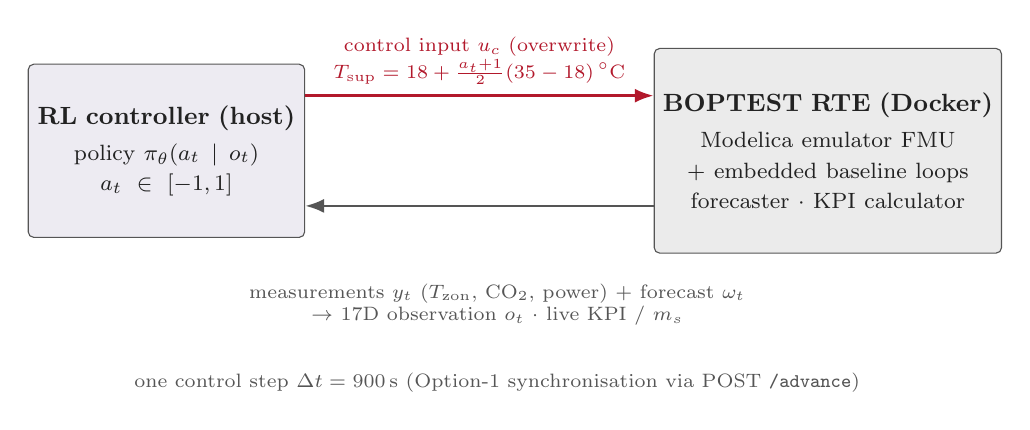
\begin{tikzpicture}[font=\small]
  \node[controller, text width=33mm, minimum height=22mm] (rl) at (0,0)
    {\textbf{RL controller (host)}\\[2pt]{\footnotesize policy $\pi_\theta(a_t\mid o_t)$}\\{\footnotesize $a_t\in[-1,1]$}};
  \node[eval, text width=42mm, minimum height=26mm] (rte) at (8.4,0)
    {\textbf{BOPTEST RTE (Docker)}\\[2pt]{\footnotesize Modelica emulator FMU}\\{\footnotesize $+$ embedded baseline loops}\\{\footnotesize forecaster $\cdot$ KPI calculator}};
  % action path (top)
  \draw[-{Latex[length=2.4mm]}, cAccurate, line width=1.1pt]
    ([yshift=7mm]rl.east) -- node[above, font=\scriptsize, text=cAccurate, align=center]
      {control input $u_c$ (overwrite)\\ $T_{\mathrm{sup}}=18+\tfrac{a_t+1}{2}(35-18)\,\degC$}
    ([yshift=7mm]rte.west);
  % measurement path (bottom). The label is placed clear of the boxes rather than on
  % the arrow: at \scriptsize it is wider than the 45mm gap and used to run under both.
  \draw[-{Latex[length=2.4mm]}, cMut, line width=1.0pt]
    ([yshift=-7mm]rte.west) -- ([yshift=-7mm]rl.east);
  \node[font=\scriptsize, text=cMut, align=center] at (4.2,-1.95)
    {measurements $y_t$ ($T_{\mathrm{zon}}$, CO$_2$, power) $+$ forecast $\omega_t$\\ $\rightarrow$ 17D observation $o_t\ \cdot$ live KPI $/\ m_s$};
  \node[font=\scriptsize, text=cMut] at (4.2,-2.95) {one control step $\Delta t=\SI{900}{\second}$ (Option-1 synchronisation via POST \texttt{/advance})};
\end{tikzpicture}
\end{document}
